\documentclass[10pt]{article}
\usepackage{graphicx}
\usepackage{algorithm}
\usepackage{hyperref}
\usepackage{algorithmic}
\usepackage[margin=1.0in]{geometry}
\usepackage{float}
\usepackage{subcaption}
\usepackage{sidecap}
\usepackage{pgffor}
\usepackage{tikz}
\usetikzlibrary{shapes, arrows}


\parskip 0.05in
\begin{document}
\title{\bf Can we predict fire with weather data?}
\author{Harsh (hp444), Yi Yao (yy899), Murali (mt788)}
\maketitle

\tableofcontents
\newpage

\section{Introduction}
The weather has literally been the hot topic of discussion in recent times.
One aspect of weather data is that, when it is combined with other data
sets, it can be used to predict varied different aspects related to
the society. For example, one particular aspect could be how does traffic
conditions change based on the weather in a particular city or if there is
a correlation between crime rates and weather conditions. In this project,
we are trying to address a more important issue of predicting wildfires in
different cities based on weather conditions. Since the future weather data
is readily available these days, a good model would help predict these
wildfires in advance and take necessary precautions to completely avoid it.
This would help avoid human and wildlife loss. It would also help contain
the impact of these wildfires on the environment which increases the
content of poisonous gases in the environment, making the nearby
uninhabitable.\par
Wildfires are growing in frequency and intensity by the day. The 2019
wildfire season of California has more than 6800 fires recorded by the US
Forest Service and approximately 250000 acres of burnt land. These
wildfires could be the result of foul human activities but there has been
a lot of speculation on the high correlation of these fires with the
weather. Climate change is not only making the fire season longer but on
average much more intense. The idea is to use the model to predict these
fires in advance, thereby reducing such incidents.\par
\section{EDA}

We have created a website to help visualize our dataset.\par 
\url{https://leafyao8621.github.io/firevisualization.github.io/}
\subsection{Covariates}
To build our final dataset, we wrote a python script to get the
geographical coordinate (latitude and longitude) of all cities and built
tables with missing information about fires. Then, we went through the
database with information about fires and filled in the fire indicator
in the tables using the coordinates obtained in the previous step.\par
The features that we have in our final dataset are:
\begin{table}[H]
    \centering
    \caption{Features}
    \begin{tabular}{l|l|l}
        Covariate &Type &Description\\\hline
        Humidity &Real &Humidity at a given hour\\
        Pressure &Real &Atmospheric Pressure at a given hour\\
        Temperature &Real &Atmospheric temperature at a given hour\\
        Weather Description &Categorical &Description of weather at
        a given time, e.g. ``sky is ckear''\\
        WindDirection &Real &Wind direction in degrees at a given time,
        North being $0^\circ$,\\
        & &clock-wise being positive direction\\
        WindSpeed &Real &Wind speed at a given time\\
    \end{tabular}
\end{table}
\begin{table}[H]
    \centering
    \caption{Response}
    \begin{tabular}{l|l|l}
        Response &Type &Description\\\hline
        Fire &Boolean &Whether there's a fire at a given hour\\
    \end{tabular}
\end{table}
\subsection{Basic Statistics}
The size of the dataset in the Fires table is: $18,800,465\times 39$,
the size of the weather table is: $1,629,108\times 10$ and
the size of the final table is: $1,629,108\times 11$. The following
figures help illustrate what the final dataset looks like:\par
\begin{figure}[H]
    \centering
    \begin{subfigure}[t]{0.48\textwidth}
        \centering
        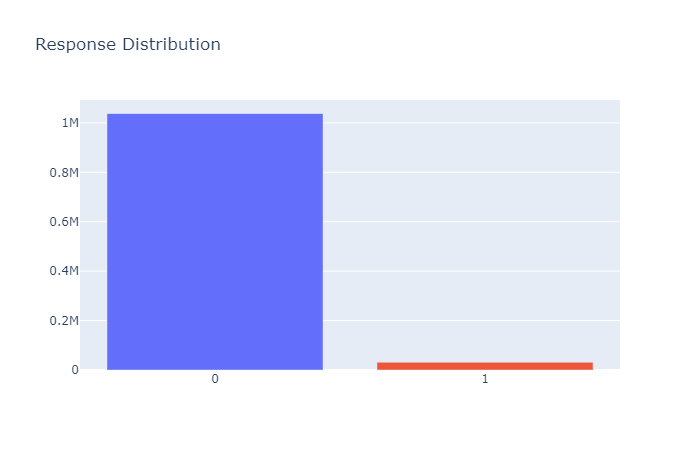
\includegraphics[width=0.8\textwidth]{../res/eda1.png}
        \caption{Response Distribution}
    \end{subfigure}
    \begin{subfigure}[t]{0.48\textwidth}
        \centering
        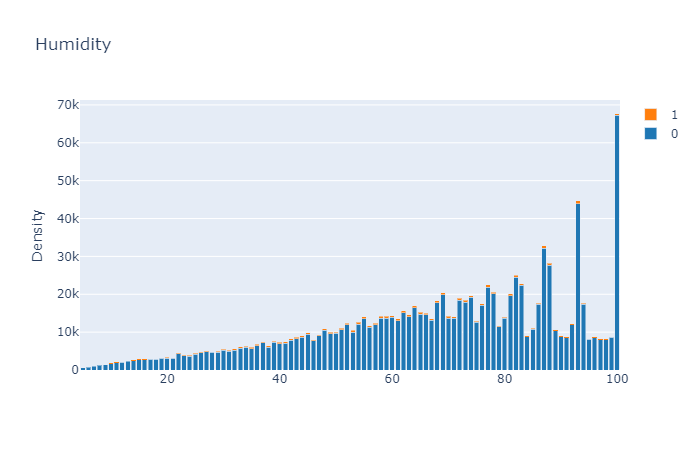
\includegraphics[width=0.8\textwidth]{../res/eda2.png}
        \caption{Histogram of Humidity}
    \end{subfigure}
    \begin{subfigure}[t]{0.48\textwidth}
        \centering
        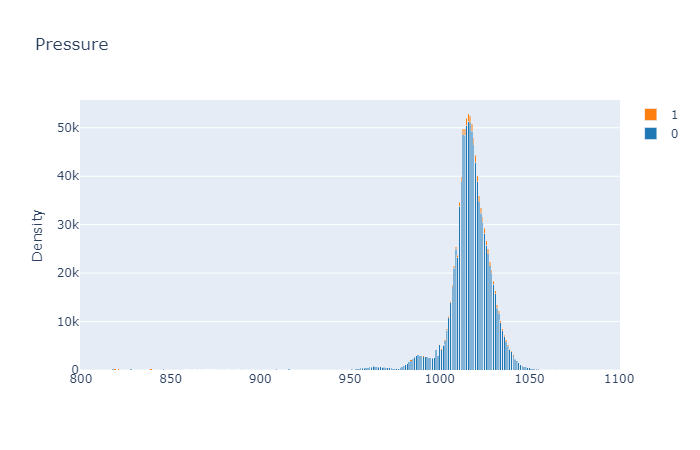
\includegraphics[width=0.8\textwidth]{../res/eda3.png}
        \caption{Histogram of Pressure}
    \end{subfigure}
    \begin{subfigure}[t]{0.48\textwidth}
        \centering
        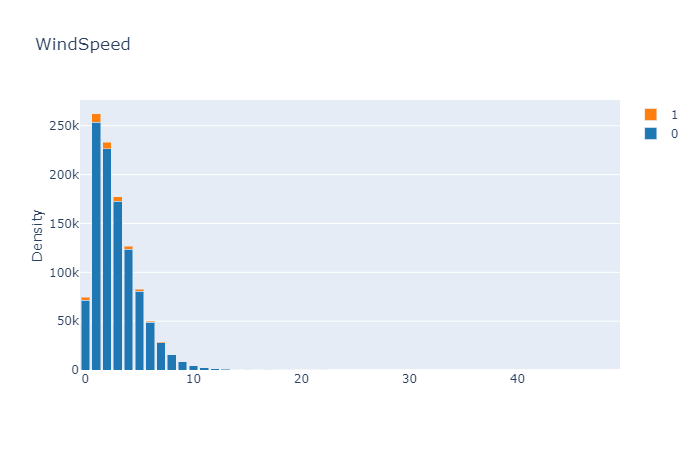
\includegraphics[width=0.8\textwidth]{../res/eda5.png}
        \caption{Histogram of Wind Speed}
    \end{subfigure}
    \caption{Visualization}
\end{figure}


\begin{figure}[H]
    \centering
    \begin{subfigure}[t]{0.3\textwidth}
        \centering
        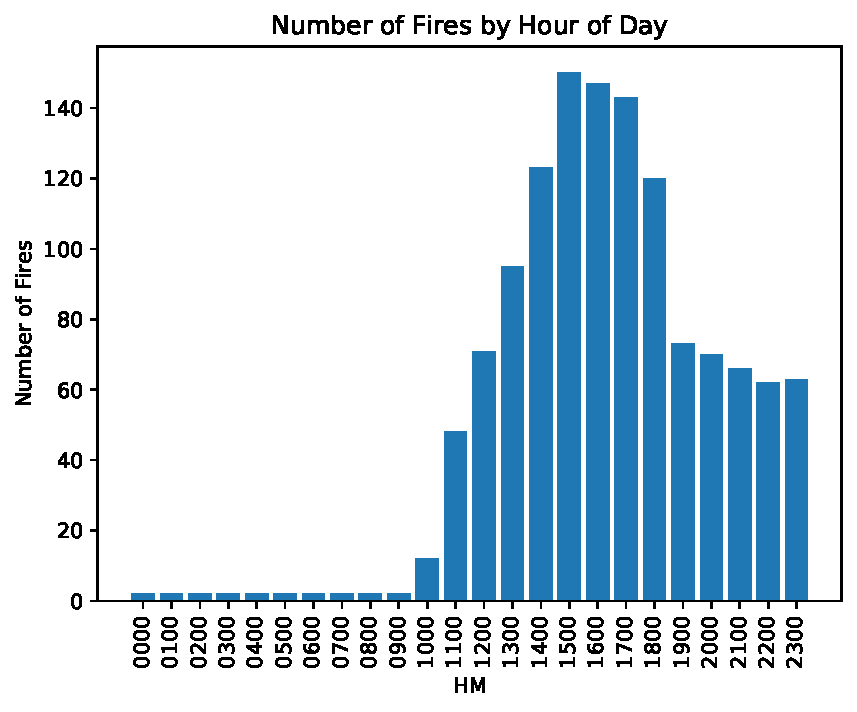
\includegraphics[width=0.8\textwidth]{../plot/byhour_sf.pdf}
        \caption{San Francisco}
    \end{subfigure}
    \begin{subfigure}[t]{0.3\textwidth}
        \centering
        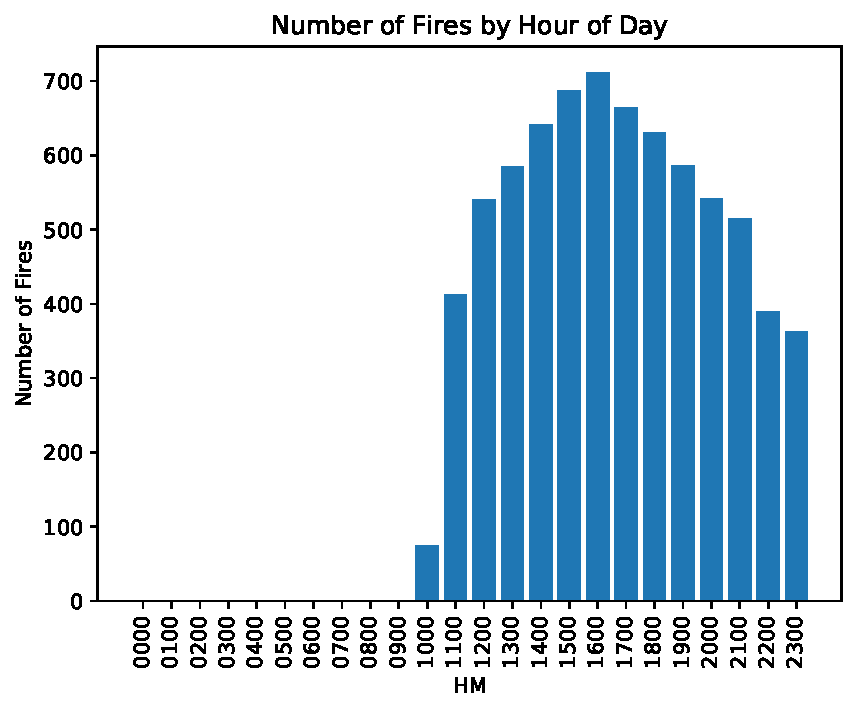
\includegraphics[width=0.8\textwidth]{../plot/byhour_ny.pdf}
        \caption{New York}
    \end{subfigure}
    \begin{subfigure}[t]{0.3\textwidth}
        \centering
        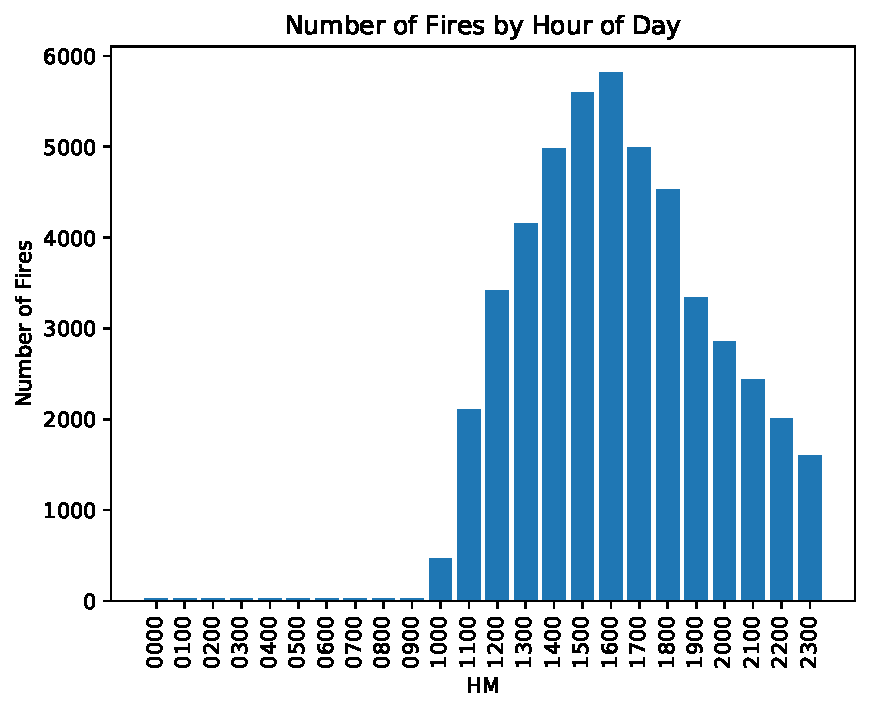
\includegraphics[width=0.8\textwidth]{../plot/byhour_all.pdf}
        \caption{All Cities}
    \end{subfigure}
    \caption{Hourly Fire Distribution}
\end{figure}

\begin{figure}[H]
    \centering
    \begin{subfigure}[t]{0.3\textwidth}
        \centering
        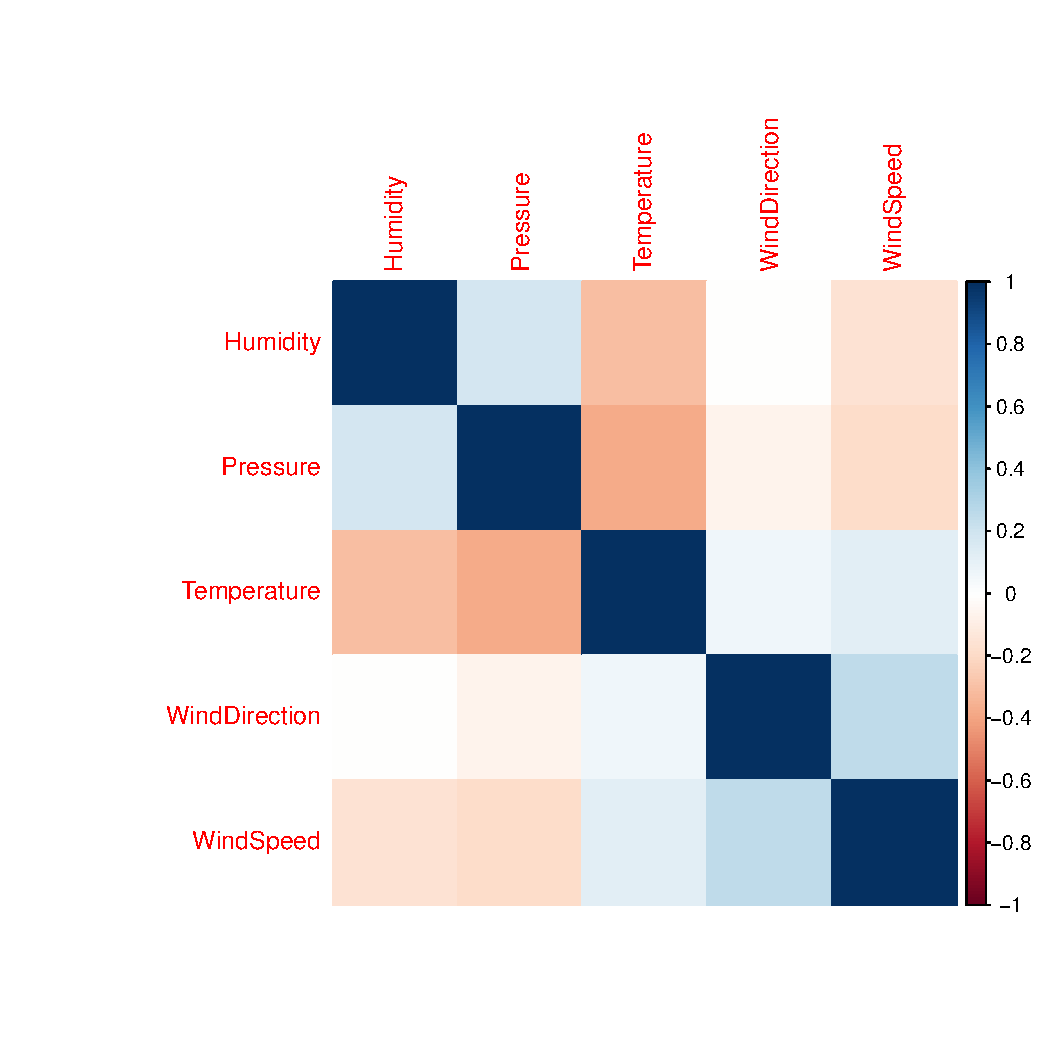
\includegraphics[width=0.8\textwidth]{../plot/corr_sf.pdf}
        \caption{San Francisco}
    \end{subfigure}
    \begin{subfigure}[t]{0.3\textwidth}
        \centering
        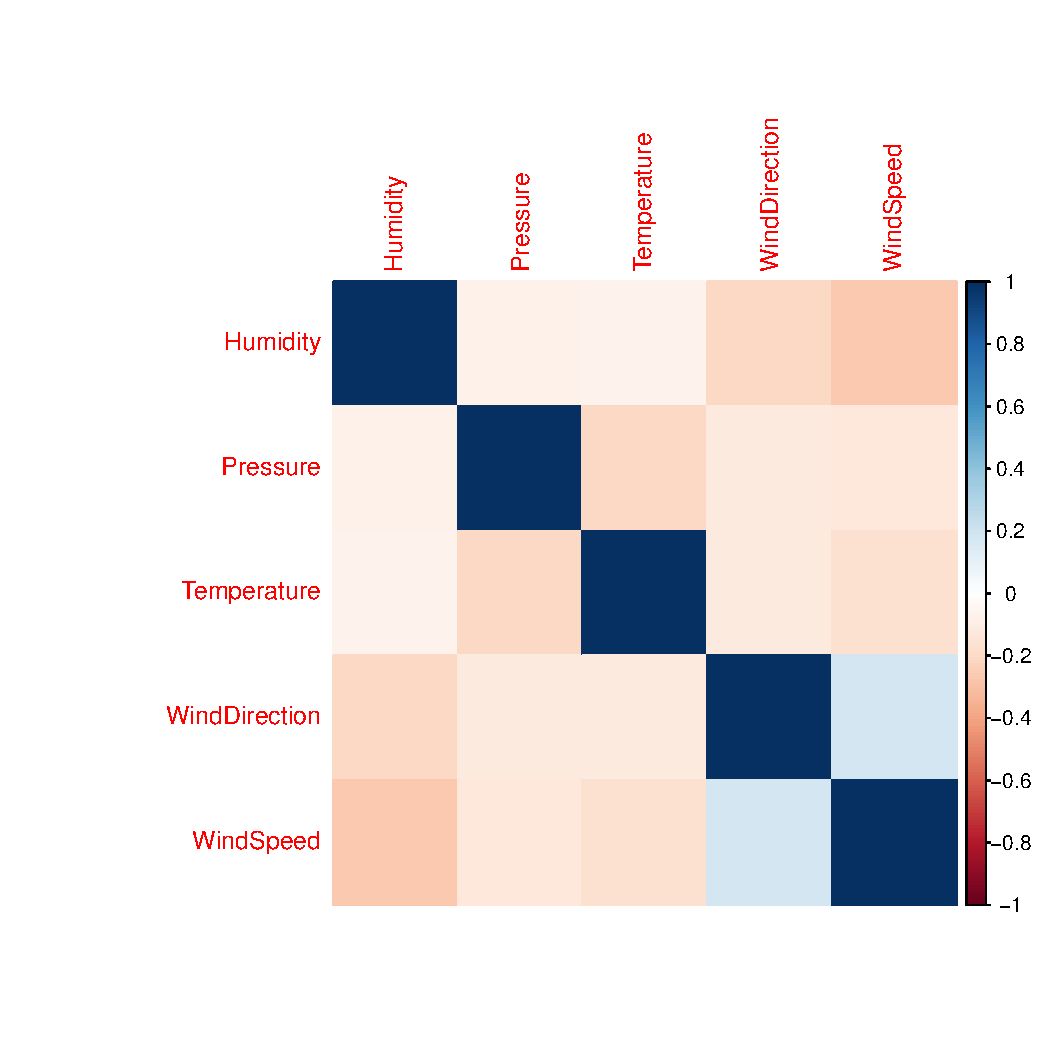
\includegraphics[width=0.8\textwidth]{../plot/corr_ny.pdf}
        \caption{New York}
    \end{subfigure}
    \begin{subfigure}[t]{0.3\textwidth}
        \centering
        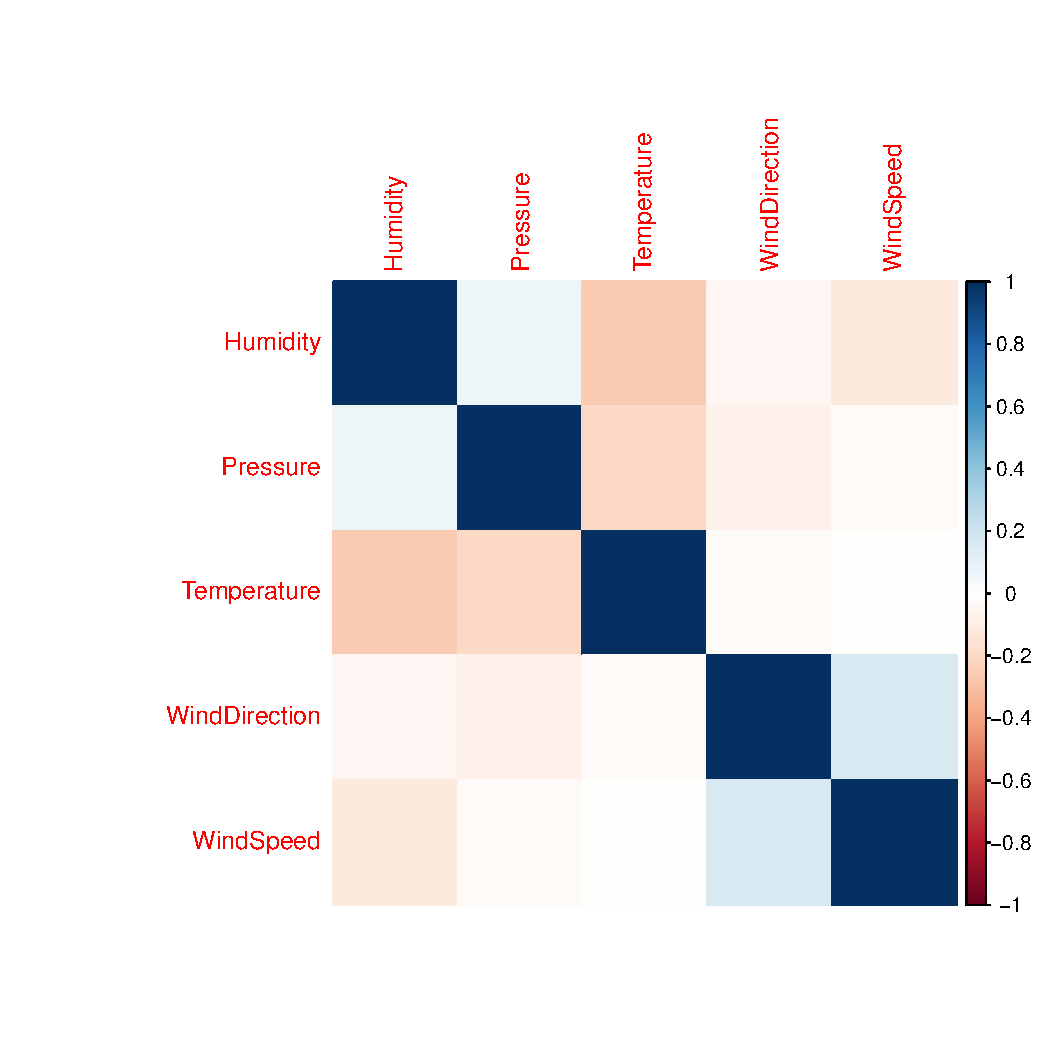
\includegraphics[width=0.8\textwidth]{../plot/corr_all.pdf}
        \caption{All Cities}
    \end{subfigure}
    \caption{Correlation Plot}
\end{figure}

\newpage

From Figure 1, we observed that we have
significantly fewer positive samples (data points where the fire indicator
has value 1) than negative samples (data points where the fire indicator
has value 0).\par

From Figure 2, we observed that very few fires are recorded in the time
span of 00:00 to 10:00, while almost all fires are recorded in the time
span of 10:00 to 23:00. We have realized that the negative samples in that
time span might be due to missing data, or people not reporting during
that time span. If we fit a hourly seasonality model, we may overfit
to data points in this time span, and end up
predicting no fire in this time span, potentially making our models
Weapons of Math Destruction.\par

From Figure 3, we observed that the correlation between features is
DIFFERENT in different cities, as well as overall, which justifies
our decision to build city-specific models.\par
\section{Brief Description of Algorithms and Definitions Used}
\subsection{XGBoost}
XGBoost is an implementation of gradient boosted decision trees designed
for speed and performance.Boosting is an ensemble technique where new
models are added to correct the errors made by existing models. Models are
added sequentially until no further improvements can be made. A popular
example is the AdaBoost algorithm that weights data points that are hard
to predict. Gradient boosting is an approach where new models are created
that predict the residuals or errors of prior models and then added
together to make the final prediction. It is called gradient boosting
because it uses a gradient descent algorithm to minimize the loss when
adding new models.\par
\subsection{SVM}
A support-vector machine constructs a hyperplane or set of hyperplanes in a
high- or infinite-dimensional space, which can be used for classification,
regression, or other tasks like outliers detection.[3] Intuitively, a good
separation is achieved by the hyperplane that has the largest distance to
the nearest training-data point of any class (so-called functional margin),
since in general the larger the margin, the lower the generalization error
of the classifier.\par
\subsection{Decision Trees}
A decision tree is a decision support tool that uses a tree-like model of
decisions and their possible consequences, including chance event outcomes,
resource costs, and utility. It is one way to display an algorithm that
only contains conditional control statements.\par
\subsection{DBScan}
DBSCAN - Density-Based Spatial Clustering of Applications with Noise.
DBScan finds core samples of high density and expands clusters from them.
It is good for data which contains clusters of similar density.
\subsection{Boosting}
Averaging predicted values from estimators trained on balanced random
subsets of data. For example, if we have a data set with 10 positive
samples and 100 negative samples, we train the estimators on multiple
balanced random sub-samples of the dataset, each containing all the 
positive samples.\par
\subsection{Balanced Accuracy}
The balanced accuracy in binary and multiclass classification problems to
deal with imbalanced datasets. It is defined as the average of recall
obtained on each class.

\section{Model Building and Accuracy Tuning}
\begin{figure}[H]
    \centering
    \tikzstyle{block} = [rectangle, draw]
\tikzstyle{line} = [draw, -latex']
\begin{tikzpicture}
    \node [block] (n0)
    {$\begin{array}{l}
        \textbf{Experiment 0}\\
        \textrm{Random Forest}\\
        \textrm{XGBoost}\\
        \textrm{SVM with RBF Kernel}\\
        \textrm{Categorical Encoding}\\
    \end{array}$};
    \node [block, right of = n0, node distance = 55mm] (n1)
    {$\begin{array}{l}
        \textbf{Experiment 1}\\
        \textrm{Random Forest}\\
        \textrm{XGBoost}\\
        \textrm{SVM with RBF Kernel}\\
        \textrm{Balanced Under-sampling}\\
        \textrm{Categorical Encoding}\\
    \end{array}$};
    \node [block, below of = n1, node distance = 30mm] (n2)
    {$\begin{array}{l}
        \textbf{Experiment 2}\\
        \textrm{Boosted Random Forest}\\
        \textrm{Boosted XGBoost}\\
        \textrm{Balanced Under-sampling}\\
        \textrm{Categorical Encoding}\\
    \end{array}$};
    \node [block, left of = n2, node distance = 53mm] (n3)
    {$\begin{array}{l}
        \textbf{Experiment 3}\\
        \textrm{Random Forest}\\
        \textrm{XGBoost}\\
        \textrm{Balanced Under-sampling}\\
        \textrm{Boosting}\\
        \textrm{Ordinal Encoding}\\
    \end{array}$};
    \node [block, below of = n3, node distance = 35mm] (n4)
    {$\begin{array}{l}
        \textbf{Experiment 4}\\
        \textrm{Random Forest}\\
        \textrm{XGBoost}\\
        \textrm{Balanced Under-sampling}\\
        \textrm{Boosting}\\
        \textrm{Ordinal Encoding}\\
        \textrm{DBScan Clustering as Feature}\\
    \end{array}$};
    \node [block, right of = n4, node distance = 60mm] (n5)
    {$\begin{array}{l}
        \textbf{Experiment 5}\\
        \textrm{XGBoost}\\
        \textrm{SVM with RBF Kernel}\\
        \textrm{Decision Tree}\\
        \textrm{Stacked Ensemble}\\
        \textrm{Balanced Under-sampling}\\
        \textrm{Ordinal Encoding}\\
        \textrm{DBScan Clustering as Feature}\\
    \end{array}$};
    \path [line] (n0) -- (n1);
    \path [line] (n1) -- (n2);
    \path [line] (n2) -- (n3);
    \path [line] (n3) -- (n4);
    \path [line] (n4) -- (n5);
\end{tikzpicture}

    \caption{Flowchart of Experiments}
\end{figure}
\subsection{Preliminary Analysis}
\begin{table}[H]
    \caption{Training and Testing Metrics}
    \centering
    \begin{tabular}{|r|r|r|r|r|r|r|r|r|}
        \hline
        Experiment &Classifier &\multicolumn{2}{|r|}{Meta Parameter}
        &Training
        &Test\\
        \hline
        \hline
        0 & &\multicolumn{2}{|r|}{n\_estimator}
        &bal\_acc
        &bal\_acc\\
        \hline
        &XGBClassifier &\multicolumn{2}{|r|}{96} &0.5167 &0.5217\\
        \hline
        &RandomForestClassifier &\multicolumn{2}{|r|}{1} &0.5813 &0.6591\\
        \hline
        \hline
        1 & &\multicolumn{2}{|r|}{n\_estimator}
        &bal\_acc
        &bal\_acc\\
        \hline
        &XGBClassifier &\multicolumn{2}{|r|}{100} &0.6654 &0.6509\\
        \hline
        &RandomForestClassifier &\multicolumn{2}{|r|}{82} &0.7039 &0.6656\\
        \hline
    \end{tabular}
\end{table}
\subsubsection{Experiment 0 - Primitive Model Fitting}
First, we fit XGBoost, Random Forest and SVM by using the entire dataset
and found the accuracy to be quite low. The low accuracy could be because
of the model overfitting. There are, afterall, 1M negative samples and
roughly 25k positive samples.\par
\begin{figure}[H]
    \centering
    \foreach \i in {1,4} {%
        \begin{subfigure}[t]{0.45\textwidth}
            \centering
            \includegraphics[width=0.8\textwidth]
            {../../analysis/yi/plot_zero_part/AlbuquerqueRandomForestClassifier_\i.pdf}
        \end{subfigure}
    }
\end{figure}
\subsubsection{Experiment 1 - Under-sampling}
Recognizing the unbalanced nature of our dataset, we created a balanced
training data set by combining all the positive samples with a random
subset of all the negative samples. Using this balanced training data set,
we fit XGBoost, Random Forest and SVM with RBF kernel. We observed a
significant improvement in test accuracy in the XGBoost and Random Forest
models; however, we have not observed any significant improvement in the
SVM models.\par
\begin{figure}[H]
    \centering
    \foreach \i in {1,4} {%
        \begin{subfigure}[t]{0.45\textwidth}
            \centering
            \includegraphics[width=0.8\textwidth]
            {../../analysis/yi/plot/AlbuquerqueRandomForestClassifier_\i.pdf}
        \end{subfigure}
    }
\end{figure}
\subsection{Accurarcy Tuning}
\begin{table}[H]
    \caption{Training and Testing Metrics}
    \centering
    \begin{tabular}{|r|r|r|r|r|r|r|r|r|}
        \hline
        Experiment &Classifier &\multicolumn{2}{|r|}{Meta Parameter}
        &Training
        &Test\\
        \hline
        \hline
        2 & &n\_boost &n\_estimator
        &bal\_acc
        &bal\_acc\\
        \hline
        &XGBClassifierBS &3 &100 &0.6636 &0.6523\\
        \hline
        &RandomForestClassifierBS &2 &95 &0.7063 &0.6911\\
        \hline
        \hline
        3 & &n\_boost &n\_estimator
        &bal\_acc
        &bal\_acc\\
        \hline
        &XGBClassifierBS &4 &96 &0.6668 &0.6551\\
        \hline
        &RandomForestClassifierBS &3 &89 &0.7031 &0.6935\\
        \hline
        \hline
        4 & &n\_boost &n\_estimator
        &bal\_acc
        &bal\_acc\\
        \hline
        &XGBClassifierBS &7 &88 &0.6634 &0.6511\\
        \hline
        &RandomForestClassifierBS &5 &74 &0.7011 &0.7035\\
        \hline
        \hline
        5 & &\multicolumn{2}{|r|}{n\_ensemble}
        &bal\_acc
        &bal\_acc\\
        \hline
        &EnsembleClassifier &\multicolumn{2}{|r|}{90} &0.7185 &0.7080\\
        \hline
        &XDSClassifier &\multicolumn{2}{|r|}{96} &0.7138 &0.7327\\
        \hline
    \end{tabular}
\end{table}
\subsubsection{Experiment 2 - Boosting Models Fitted with Balanced
               Sub-samples}
Having the possibility of underfitting due to under-sampling in mind, we
have experimented with boosting to increase accuracy. By keeping all the
positive samples and randomly resampling negative samples equal to the
number of positive samples, we have kept the balance of the training data
set while making better use of the data set we have available.\par
\begin{figure}[H]
    \centering
    \foreach \i in {1,4} {%
        \begin{subfigure}[t]{0.45\textwidth}
            \centering
            \includegraphics[width=0.8\textwidth]
            {../../analysis/yi/classify_boost/plot/AlbuquerqueRandomForestClassifierBS_\i.pdf}
        \end{subfigure}
    }
\end{figure}
\subsubsection{Experiment 3 - Clusters of Many-hot Encoding}
Having observed some order in the covariate ``Weather Description'', we
have experimented with many-hot encoding for ordinal variables. Since an
overall order could not be established, we have turned to many-hot
encoding on 3 clusters of levels and one-hot encoding on the remaining
levels. As for models, we continued to use the boosted algorithms in the
previous experiment.\par
\begin{figure}[H]
    \centering
    \foreach \i in {1,4} {%
        \begin{subfigure}[t]{0.45\textwidth}
            \centering
            \includegraphics[width=0.8\textwidth]
            {../../analysis/yi/classify_boost_multiordinal/plot/AlbuquerqueRandomForestClassifierBS_\i.pdf}
        \end{subfigure}
    }
\end{figure}
\subsubsection{Experiment 4 - DBScan Clustering as Feature}
We have also experimented adding one-hot encoded output of an unsupervised
clustering algorithm, DBScan as covariates to the dataset to be fitted with
supervised models. As for models, we continued to use the boosted
algorithms in the previous experiment.\par
\begin{figure}[H]
    \centering
    \foreach \i in {1,4} {%
        \begin{subfigure}[t]{0.45\textwidth}
            \centering
            \includegraphics[width=0.8\textwidth]
            {../../analysis/yi/classify_boost_multiordinal/plot/AlbuquerqueRandomForestClassifierBS_\i.pdf}
        \end{subfigure}
    }
\end{figure}
\subsubsection{Experiment 5 - Stacked Ensemble}
In this experiment, we explore feature engineering through the addition of
two features, one which is to use the weather types as oridinal features
and another one by grouping them using DBScan Algorithm and using their
groups as features. We tried to utilize the power of ensemble learning
where we combine various weak learners in order to make better
predictions. The algorithms that we picked are SVMs with RBF Kernel,
Decision trees and XGBoost. These were identified to perform poorly with
the original dataset fed as a whole.\par
\begin{figure}[H]
    \centering
    \foreach \i in {1,4} {%
        \begin{subfigure}[t]{0.45\textwidth}
            \centering
            \includegraphics[width=0.8\textwidth]
            {../../analysis/yi/classify_xds/plot/AlbuquerqueXDSClassifier_\i.pdf}
        \end{subfigure}
    }
\end{figure}


\section{Conclusion}
Overall, our objective was to be able to predict fires given weather data.
Our accuracy depended upon the methods we picked to push the accuracy up.
We identify that we hit the information ``roof'' when it comes to how well
we could predict the fire. Some other interesting observations are as
follows:\par
\begin{enumerate}
    \item[$\ast$]
    The XGBoost algorithm when fed with one round of undersampling with
    the no. of estimators higher than 25 seemed to have learned all the
    information available.
    \item[$\ast$]
    The stacked ensemble algorithm performed the best for the cities shown
    in this report. It's interesting to note that although weak learners
    do not capture complex information, when we differ the way they
    capture that information, we see that they perform well collectively
    without having to weigh it in the final prediction.
    \item[$\ast$]
    The information roof that we clearly hit which may indicate that we
    needed more real features that inherently affect the prediction. That
    may be the error that we seem not able to avoid.
    \item[$\ast$]
    Incorrectly predicting that a city will not have an occurence of
    fire may lead to unpreparedness on the part of the fire services
    which will further cause data points to pop up as ``fire'' until our
    model really learns that there are a lot of fires. Our project may
    in this sense a weapon of math destruction. This problem can be 
    overcome by including many more features, more intelligible data and
    bumping up the accuracy to an acceptable level.
    \item[$\ast$]
    Since we have built a complete tool-chain from data-cleaning to
    automated parameter selection, we are willing to use it in production
    given that the company continues to use the same data sources.
\end{enumerate}
\newpage
\nocite{*}
\bibliographystyle{acm}
\bibliography{references}
\end{document}
